\documentclass[twocolumn]{ltjsarticle}
\usepackage{graphicx}
\setlength{\columnseprule}{0.4pt}
\title{2段組の文書}
\author{山田 太郎}
\date{\today}
\begin{document}
\maketitle
\section{2段組の文書}
図や表を挿入するときだけ2段組を解除することができます。例えば、図を挿入してみます。
\begin{figure*}[htbp]
  \centering
  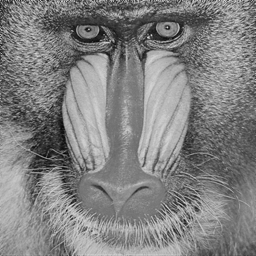
\includegraphics[scale = 0.5]{mandrill.png}
  \caption{mandrill.png}
  \label{fig:Mandrill}
\end{figure*}
さらに、表も挿入してみましょう。
\begin{table*}[htbp]
  \caption{各試験の点数}
  \label{tab:score}
  \centering
  \begin{tabular}{|l||c|c|c|c|}
    \hline
    名前／科目 & 国語 & 数学 & 理科 & 社会 \\
    \hline \hline
    田中 太郎 & 30 & 65 & 80 & 70 \\
    \hline
    佐藤 次郎 & 91 & 74 & 95 & 12 \\
    \hline
    鈴木 花子 & 84 & 98 & 100 & 68 \\
    \hline
  \end{tabular}
\end{table*}
\end{document}

